\documentclass{article}\usepackage[]{graphicx}\usepackage[]{color}
%% maxwidth is the original width if it is less than linewidth
%% otherwise use linewidth (to make sure the graphics do not exceed the margin)
\makeatletter
\def\maxwidth{ %
  \ifdim\Gin@nat@width>\linewidth
    \linewidth
  \else
    \Gin@nat@width
  \fi
}
\makeatother

\definecolor{fgcolor}{rgb}{0.345, 0.345, 0.345}
\newcommand{\hlnum}[1]{\textcolor[rgb]{0.686,0.059,0.569}{#1}}%
\newcommand{\hlstr}[1]{\textcolor[rgb]{0.192,0.494,0.8}{#1}}%
\newcommand{\hlcom}[1]{\textcolor[rgb]{0.678,0.584,0.686}{\textit{#1}}}%
\newcommand{\hlopt}[1]{\textcolor[rgb]{0,0,0}{#1}}%
\newcommand{\hlstd}[1]{\textcolor[rgb]{0.345,0.345,0.345}{#1}}%
\newcommand{\hlkwa}[1]{\textcolor[rgb]{0.161,0.373,0.58}{\textbf{#1}}}%
\newcommand{\hlkwb}[1]{\textcolor[rgb]{0.69,0.353,0.396}{#1}}%
\newcommand{\hlkwc}[1]{\textcolor[rgb]{0.333,0.667,0.333}{#1}}%
\newcommand{\hlkwd}[1]{\textcolor[rgb]{0.737,0.353,0.396}{\textbf{#1}}}%
\let\hlipl\hlkwb

\usepackage{framed}
\makeatletter
\newenvironment{kframe}{%
 \def\at@end@of@kframe{}%
 \ifinner\ifhmode%
  \def\at@end@of@kframe{\end{minipage}}%
  \begin{minipage}{\columnwidth}%
 \fi\fi%
 \def\FrameCommand##1{\hskip\@totalleftmargin \hskip-\fboxsep
 \colorbox{shadecolor}{##1}\hskip-\fboxsep
     % There is no \\@totalrightmargin, so:
     \hskip-\linewidth \hskip-\@totalleftmargin \hskip\columnwidth}%
 \MakeFramed {\advance\hsize-\width
   \@totalleftmargin\z@ \linewidth\hsize
   \@setminipage}}%
 {\par\unskip\endMakeFramed%
 \at@end@of@kframe}
\makeatother

\definecolor{shadecolor}{rgb}{.97, .97, .97}
\definecolor{messagecolor}{rgb}{0, 0, 0}
\definecolor{warningcolor}{rgb}{1, 0, 1}
\definecolor{errorcolor}{rgb}{1, 0, 0}
\newenvironment{knitrout}{}{} % an empty environment to be redefined in TeX

\usepackage{alltt}

\title{Problem Set 2}
\author{Klint Kanopka \\ EDUC 252L}
\IfFileExists{upquote.sty}{\usepackage{upquote}}{}
\begin{document}
\maketitle
\section{Breaking the Classical Test Theory Model}

  \subsection{Coin Flips}
    Coin flips should not be reliable data - they're random!  To look at this a little more analytically:
    
      \[ \alpha = \frac{K}{K-1}\Bigg(1-\frac{\sum_{i=1}^{K}p_i(1-p_i)}{\sigma_{X}^{2}}\Bigg)\]
    
    The interesting thing to note here is that the probability of flipping heads is:
      \[p_i = 0.5 \]
    And the variance on the sum of $K$ coin flips will be:
      \[ \sigma_X = 0.25K \]
    Substituting in the formula for Cronbach's Alpha:
      \[ \alpha = \frac{K}{K-1}\Bigg(1-\frac{\sum_{i=1}^{K}(0.5)(1-0.5)}{0.25K}\Bigg)\]
    Cleaning up:
      \[ \alpha = \frac{K}{K-1}\Bigg(1-\frac{0.25K}{0.25K}\Bigg)\]
      \[ \alpha = \frac{K}{K-1}(1-1)\]
      \[ \alpha = 0 \]
    The expectation, then, is that $\alpha$ shoudl be zero for each situation.


\begin{knitrout}
\definecolor{shadecolor}{rgb}{0.969, 0.969, 0.969}\color{fgcolor}
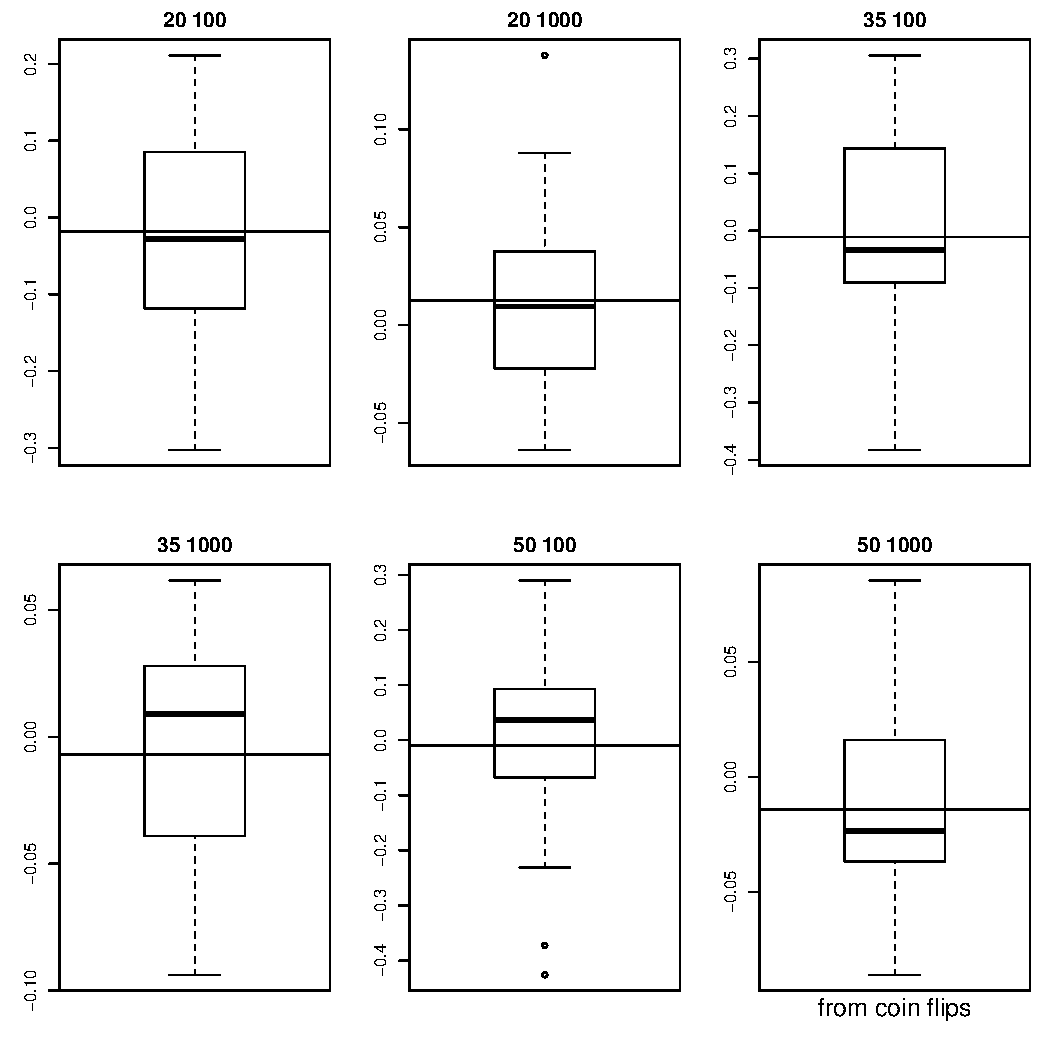
\includegraphics[width=\maxwidth]{figure/unnamed-chunk-1-1} 

\end{knitrout}

    These $\alpha$ plots make sense - they are centered around zero, as predicted.

  \subsection{Simulating Item Response Data}

\begin{knitrout}
\definecolor{shadecolor}{rgb}{0.969, 0.969, 0.969}\color{fgcolor}\begin{kframe}
\begin{alltt}
\hlcom{###################################################################################################################}
\hlcom{##now, we were kind of cheating with the coins. we didn't really impose any structure on the thing and this isn't really demonstrating something too weird about ctt, just that coin flips aren't reliable measures!}

\hlcom{##let's give ourselves a stiffer challenge. let's generate item response data that has}
\hlcom{##A. a pre-specified reliability}
\hlcom{##B. and yet weird inter-workings such that reliability estimates fall apart completely}
\hlcom{##C. [i don't really emphasize this in the below, but you can also pick (roughly) the distribution of item p-values]}
\hlcom{##below i'm going to do just that using this function.}
\hlstd{sim_ctt}\hlkwb{<-}\hlkwa{function}\hlstd{(}\hlkwc{N.items}\hlstd{,} \hlcom{#N.items needs to be even}
                  \hlkwc{N.ppl}\hlstd{,}
                  \hlkwc{s2.true}\hlstd{,}
                  \hlkwc{s2.error}\hlstd{,}
                  \hlkwc{check}\hlstd{=}\hlnum{FALSE} \hlcom{#this will produce a figure that you can use to check that things are working ok}
                  \hlstd{) \{}
    \hlcom{##desired reliability}
    \hlstd{reliability}\hlkwb{<-}\hlstd{(s2.true)}\hlopt{/}\hlstd{(s2.error}\hlopt{+}\hlstd{s2.true)}
    \hlcom{##sample (unobserved) true abilities & errors}
    \hlstd{T}\hlkwb{<-}\hlkwd{round}\hlstd{(}\hlkwd{rnorm}\hlstd{(N.ppl,}\hlkwc{mean}\hlstd{=}\hlkwd{round}\hlstd{(N.items}\hlopt{/}\hlnum{2}\hlstd{),}\hlkwc{sd}\hlstd{=}\hlkwd{sqrt}\hlstd{(s2.true)))}
    \hlstd{E}\hlkwb{<-}\hlkwd{round}\hlstd{(}\hlkwd{rnorm}\hlstd{(N.ppl,}\hlkwc{mean}\hlstd{=}\hlnum{0}\hlstd{,}\hlkwc{sd}\hlstd{=}\hlkwd{sqrt}\hlstd{(s2.error)))}
    \hlstd{O}\hlkwb{<-}\hlstd{T}\hlopt{+}\hlstd{E}
    \hlkwd{ifelse}\hlstd{(O}\hlopt{<}\hlnum{0}\hlstd{,}\hlnum{0}\hlstd{,O)}\hlkwb{->}\hlstd{O}
    \hlkwd{ifelse}\hlstd{(O}\hlopt{>}\hlstd{N.items,N.items,O)}\hlkwb{->}\hlstd{O}
    \hlcom{##note that we already know how many items a person got right (O)}
    \hlcom{##ctt doesn't specify how individual item responses are generated.}
    \hlcom{##so we have carte blance in terms of coming up with item responses. here's how i'm going to do it. }
    \hlstd{pr}\hlkwb{<-}\hlkwd{runif}\hlstd{(N.items,}\hlkwc{min}\hlstd{=}\hlnum{.25}\hlstd{,}\hlkwc{max}\hlstd{=}\hlnum{.85}\hlstd{)}
    \hlstd{pr.interval}\hlkwb{<-}\hlkwd{c}\hlstd{(}\hlnum{0}\hlstd{,}\hlkwd{cumsum}\hlstd{(pr))}\hlopt{/}\hlkwd{sum}\hlstd{(pr)}
    \hlstd{resp}\hlkwb{<-}\hlkwd{list}\hlstd{()}
    \hlkwa{for} \hlstd{(i} \hlkwa{in} \hlnum{1}\hlopt{:}\hlstd{N.ppl) \{} \hlcom{#for each person}
        \hlstd{resp.i}\hlkwb{<-}\hlkwd{rep}\hlstd{(}\hlnum{0}\hlstd{,N.items)} \hlcom{#start them with all 0s}
        \hlkwa{if} \hlstd{(O[i]}\hlopt{>}\hlnum{0}\hlstd{) \{}
            \hlkwa{for} \hlstd{(j} \hlkwa{in} \hlnum{1}\hlopt{:}\hlstd{O[i]) \{} \hlcom{#now for each of the observed correct responses (for those who got at least 1 item right) i'll pick an item to mark correct}
                \hlstd{init.val}\hlkwb{<-}\hlnum{1}
                \hlkwa{while} \hlstd{(init.val}\hlopt{==}\hlnum{1}\hlstd{) \{}
                    \hlstd{index}\hlkwb{<-}\hlkwd{cut}\hlstd{(}\hlkwd{runif}\hlstd{(}\hlnum{1}\hlstd{),pr.interval,}\hlkwc{labels}\hlstd{=}\hlnum{FALSE}\hlstd{)} \hlcom{#here i pick the item wherein i weight the items by the "pr" argument that is random here but could be pre-specied by the user}
                    \hlstd{init.val}\hlkwb{<-}\hlstd{resp.i[index]}
                \hlstd{\}}
                \hlstd{resp.i[index]}\hlkwb{<-}\hlnum{1}
            \hlstd{\}}
        \hlstd{\}}
        \hlstd{resp[[i]]}\hlkwb{<-}\hlstd{resp.i}
    \hlstd{\}}
    \hlkwd{do.call}\hlstd{(}\hlstr{"rbind"}\hlstd{,resp)}\hlkwb{->}\hlstd{resp}
    \hlcom{##note that we are getting both the p-values and the true score/observed score relationships right!}
    \hlkwa{if} \hlstd{(check) \{}
        \hlkwd{par}\hlstd{(}\hlkwc{mfrow}\hlstd{=}\hlkwd{c}\hlstd{(}\hlnum{2}\hlstd{,}\hlnum{1}\hlstd{))}
        \hlkwd{plot}\hlstd{(T,}\hlkwd{rowSums}\hlstd{(resp),}\hlkwc{xlab}\hlstd{=}\hlstr{"true score"}\hlstd{,}\hlkwc{ylab}\hlstd{=}\hlstr{"observed scores"}\hlstd{);} \hlkwd{abline}\hlstd{(}\hlnum{0}\hlstd{,}\hlnum{1}\hlstd{)}
        \hlkwd{plot}\hlstd{(pr,}\hlkwd{colMeans}\hlstd{(resp),}\hlkwc{xlab}\hlstd{=}\hlstr{"pr"}\hlstd{,}\hlkwc{ylab}\hlstd{=}\hlstr{"observed p-values"}\hlstd{);} \hlkwd{abline}\hlstd{(}\hlnum{0}\hlstd{,}\hlnum{1}\hlstd{)}
    \hlstd{\}}
    \hlstd{obs.rel}\hlkwb{<-}\hlkwd{cor}\hlstd{(T,O)}\hlopt{^}\hlnum{2} \hlcom{#we can use this to make sure that the true and observed score variances are right.}
    \hlkwd{print}\hlstd{(}\hlkwd{c}\hlstd{(reliability,obs.rel))} \hlcom{##for real time checking, these are the pre-specified reliability and what we get from correlation our true and observed scores}
    \hlstd{kr}\hlkwb{<-}\hlkwd{kr20}\hlstd{(resp)}
    \hlkwd{c}\hlstd{(obs.rel,kr)}
\hlstd{\}}

\hlcom{##to illustrate the basic idea here, we'll generate 10 sets of item response data.}
\hlcom{##for each iteration, we'll use the same parameters, these are below.}
\hlstd{N.items}\hlkwb{<-}\hlnum{50}
\hlstd{N.ppl}\hlkwb{<-}\hlnum{500}
\hlstd{s2.true}\hlkwb{<-}\hlnum{10}
\hlstd{s2.error}\hlkwb{<-}\hlnum{3}
\hlstd{alph}\hlkwb{<-}\hlkwd{list}\hlstd{()}
\hlkwa{for} \hlstd{(i} \hlkwa{in} \hlnum{1}\hlopt{:}\hlnum{10}\hlstd{) \{}
    \hlstd{alph[[i]]}\hlkwb{<-}\hlkwd{sim_ctt}\hlstd{(}\hlkwc{N.items}\hlstd{=N.items,}\hlkwc{N.ppl}\hlstd{=N.ppl,}\hlkwc{s2.true}\hlstd{=s2.true,}\hlkwc{s2.error}\hlstd{=s2.error,}\hlkwc{check}\hlstd{=}\hlnum{TRUE}\hlstd{)} \hlcom{#note, the check option is goign to produce a figure that allows us to check the marginals to make sure things are looking ok}
\hlstd{\}}
\end{alltt}
\end{kframe}
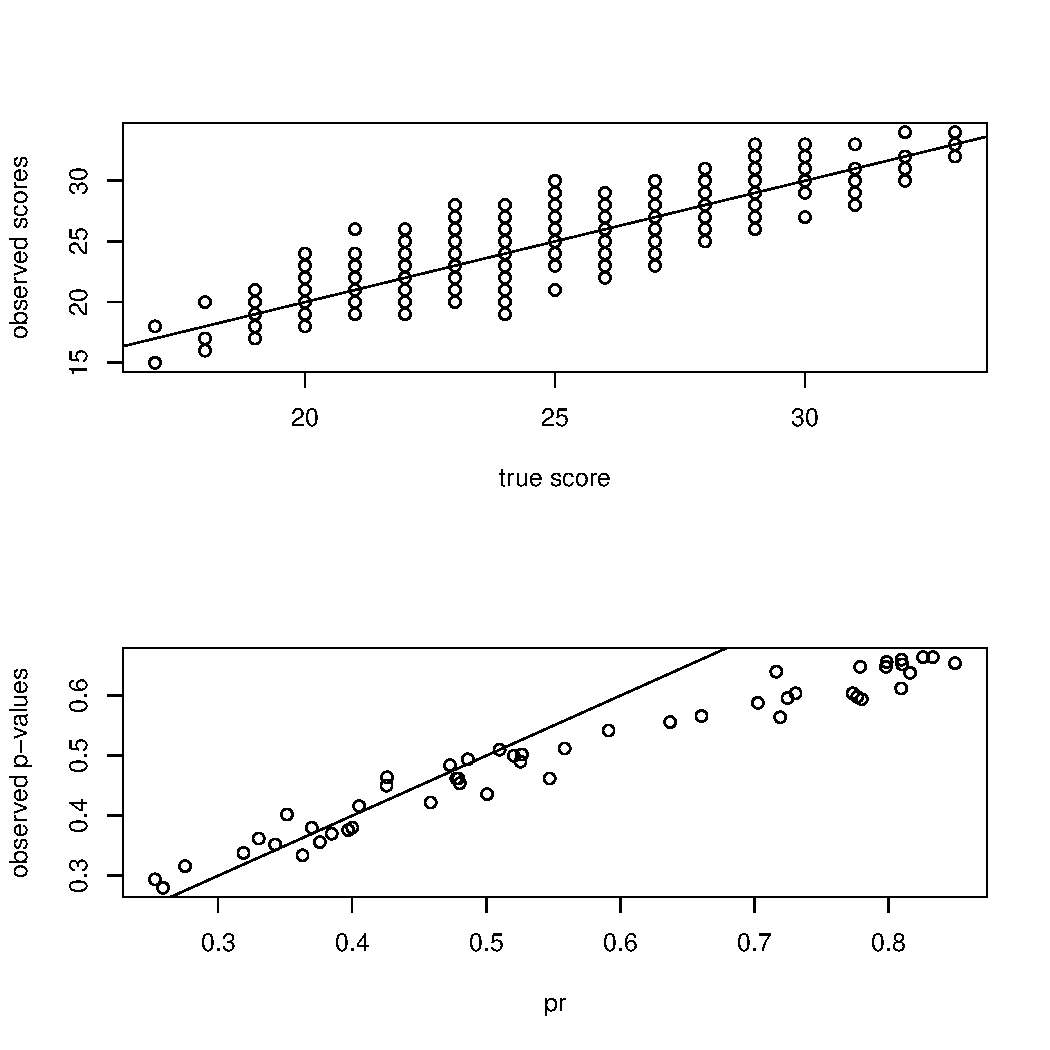
\includegraphics[width=\maxwidth]{figure/unnamed-chunk-2-1} 
\begin{kframe}\begin{verbatim}
## [1] 0.7692308 0.7519898
\end{verbatim}
\end{kframe}
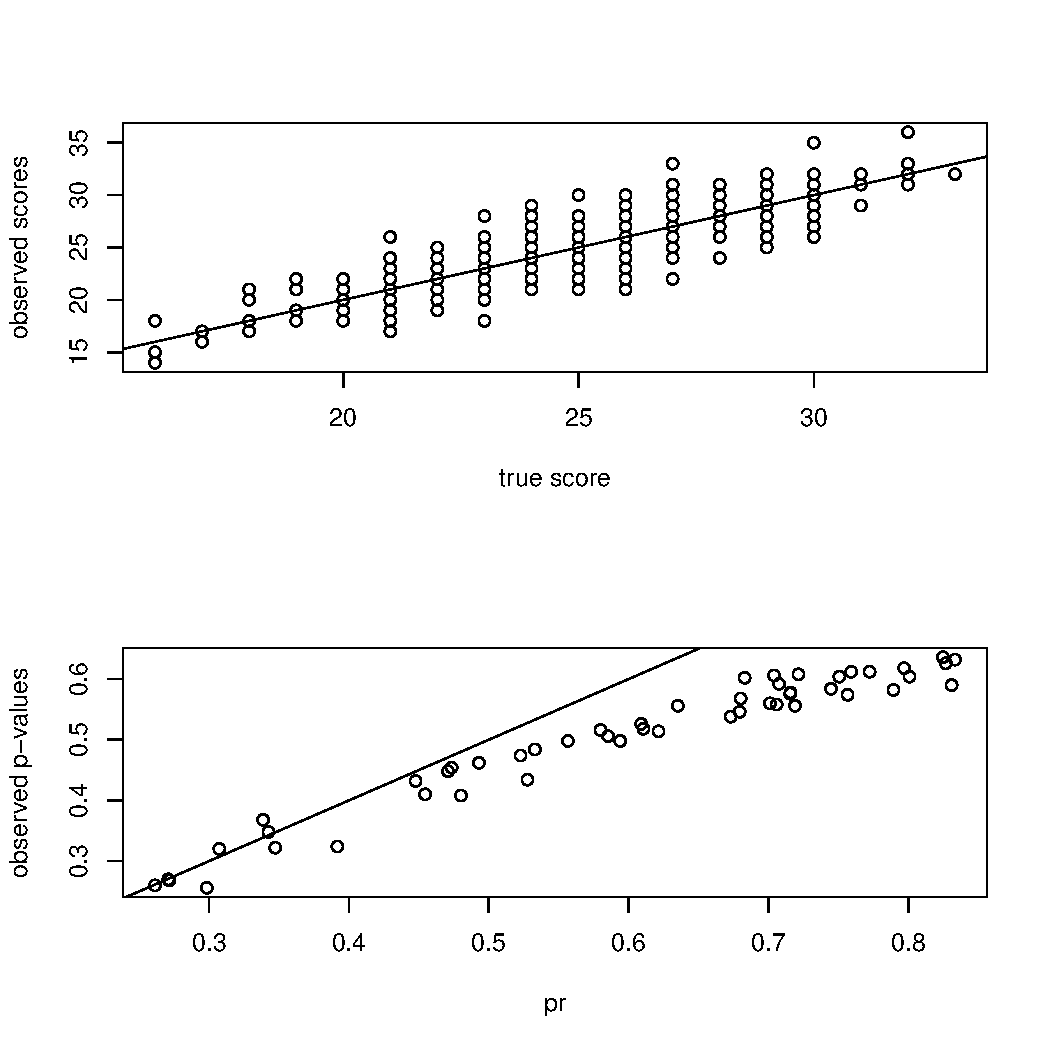
\includegraphics[width=\maxwidth]{figure/unnamed-chunk-2-2} 
\begin{kframe}\begin{verbatim}
## [1] 0.7692308 0.7586454
\end{verbatim}
\end{kframe}
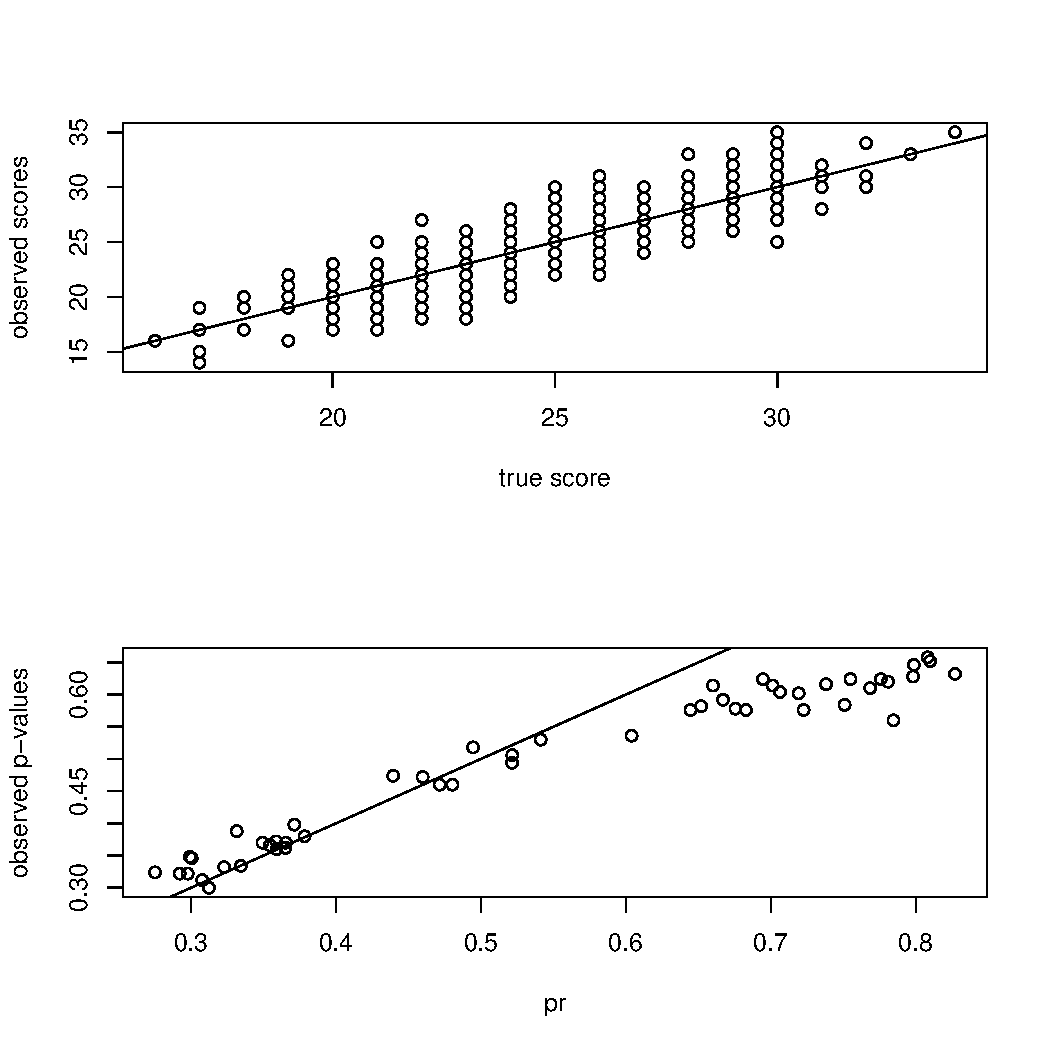
\includegraphics[width=\maxwidth]{figure/unnamed-chunk-2-3} 
\begin{kframe}\begin{verbatim}
## [1] 0.7692308 0.7453799
\end{verbatim}
\end{kframe}
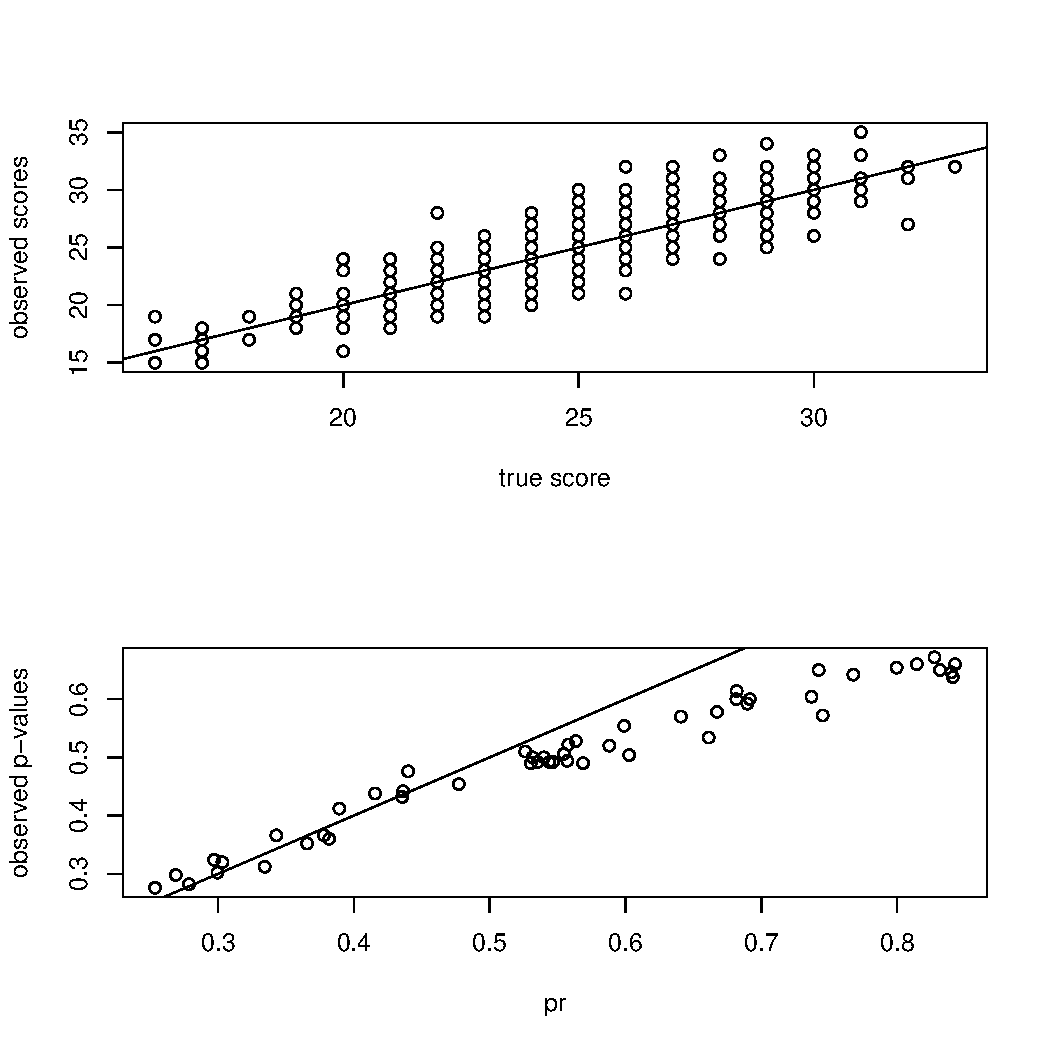
\includegraphics[width=\maxwidth]{figure/unnamed-chunk-2-4} 
\begin{kframe}\begin{verbatim}
## [1] 0.7692308 0.7847733
\end{verbatim}
\end{kframe}
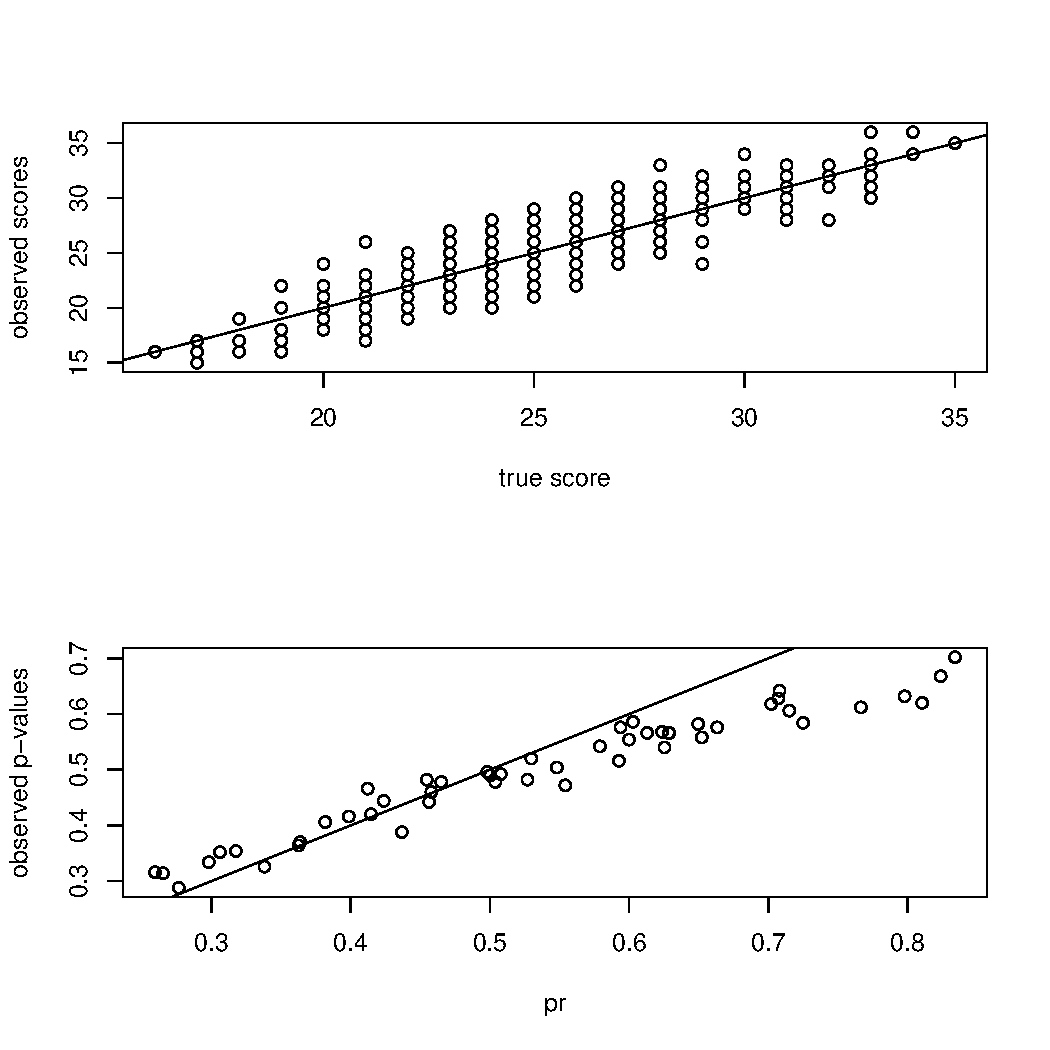
\includegraphics[width=\maxwidth]{figure/unnamed-chunk-2-5} 
\begin{kframe}\begin{verbatim}
## [1] 0.7692308 0.7415703
\end{verbatim}
\end{kframe}
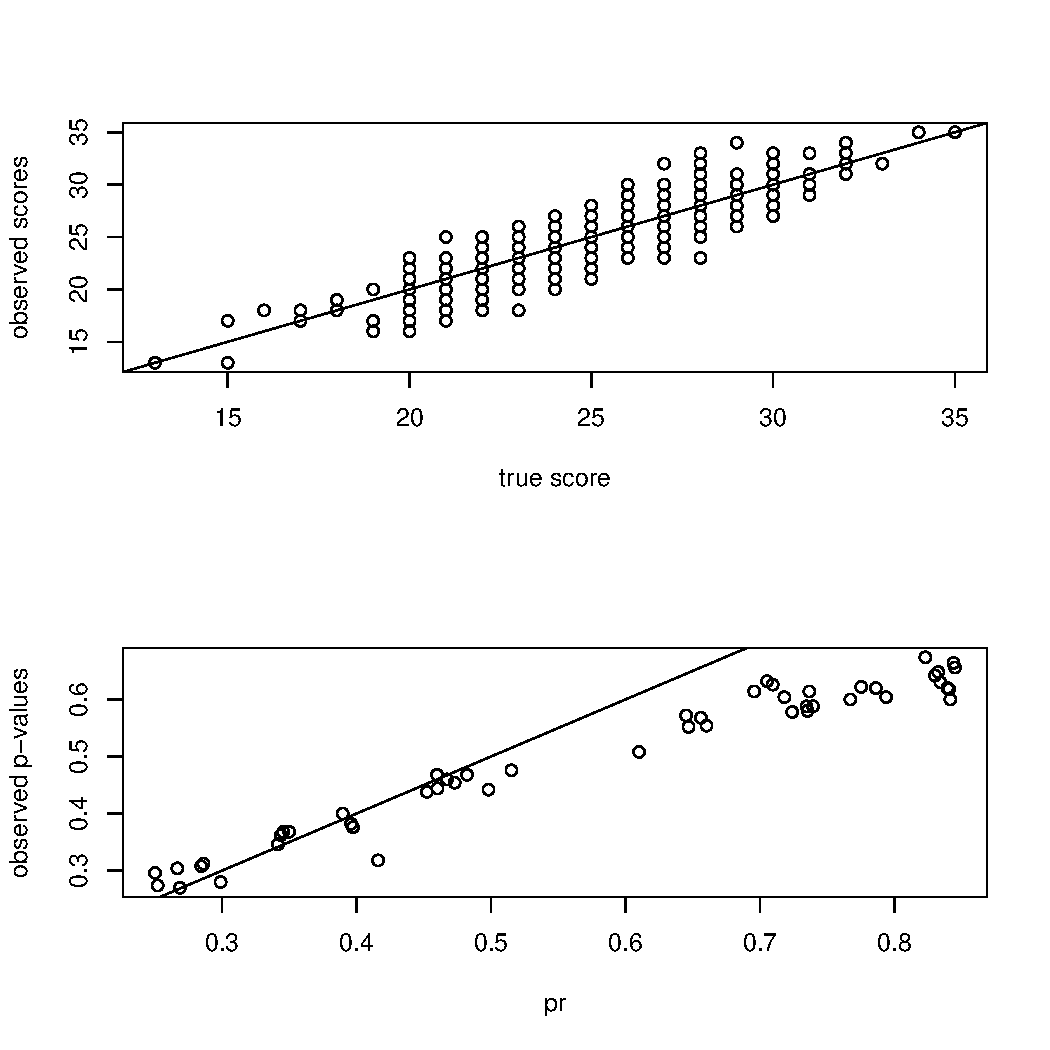
\includegraphics[width=\maxwidth]{figure/unnamed-chunk-2-6} 
\begin{kframe}\begin{verbatim}
## [1] 0.7692308 0.7627290
\end{verbatim}
\end{kframe}
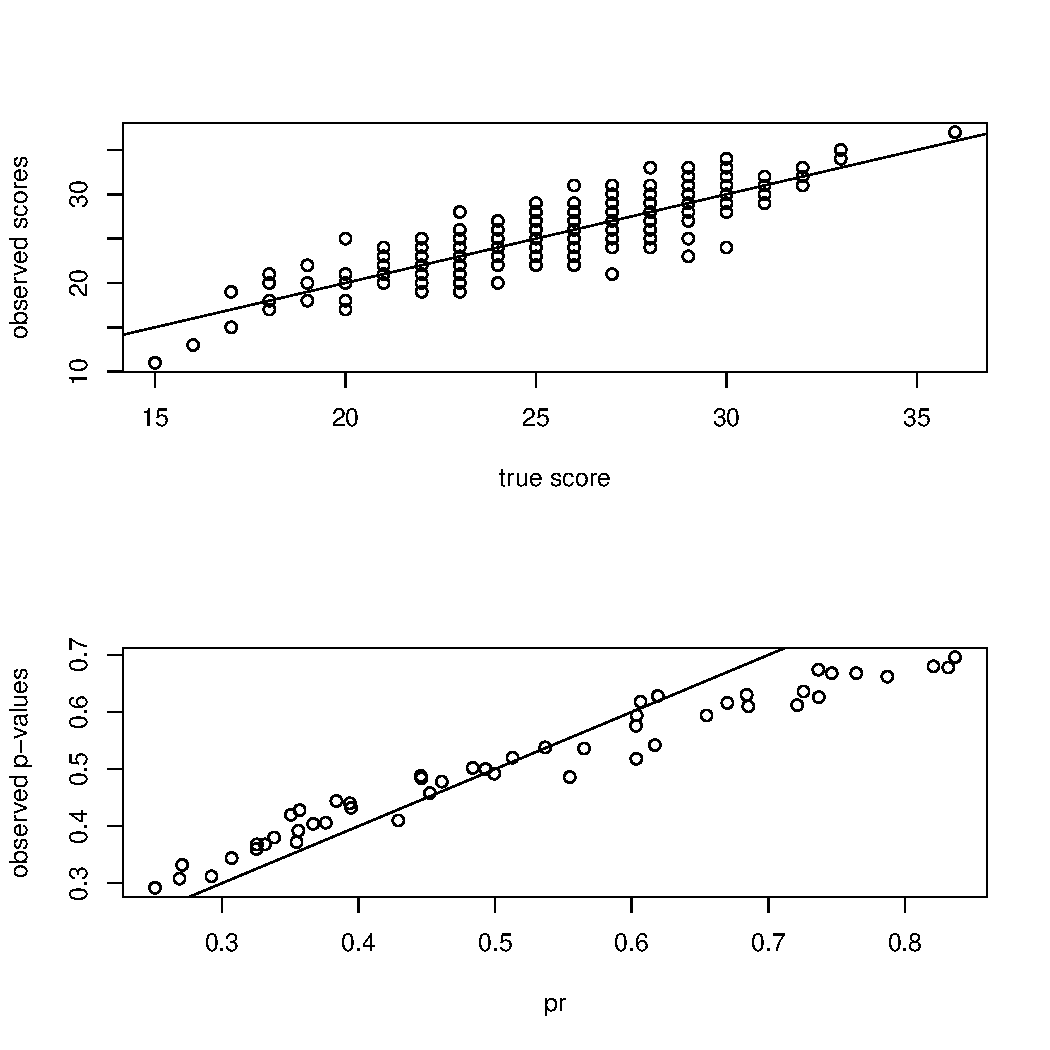
\includegraphics[width=\maxwidth]{figure/unnamed-chunk-2-7} 
\begin{kframe}\begin{verbatim}
## [1] 0.7692308 0.7436331
\end{verbatim}
\end{kframe}
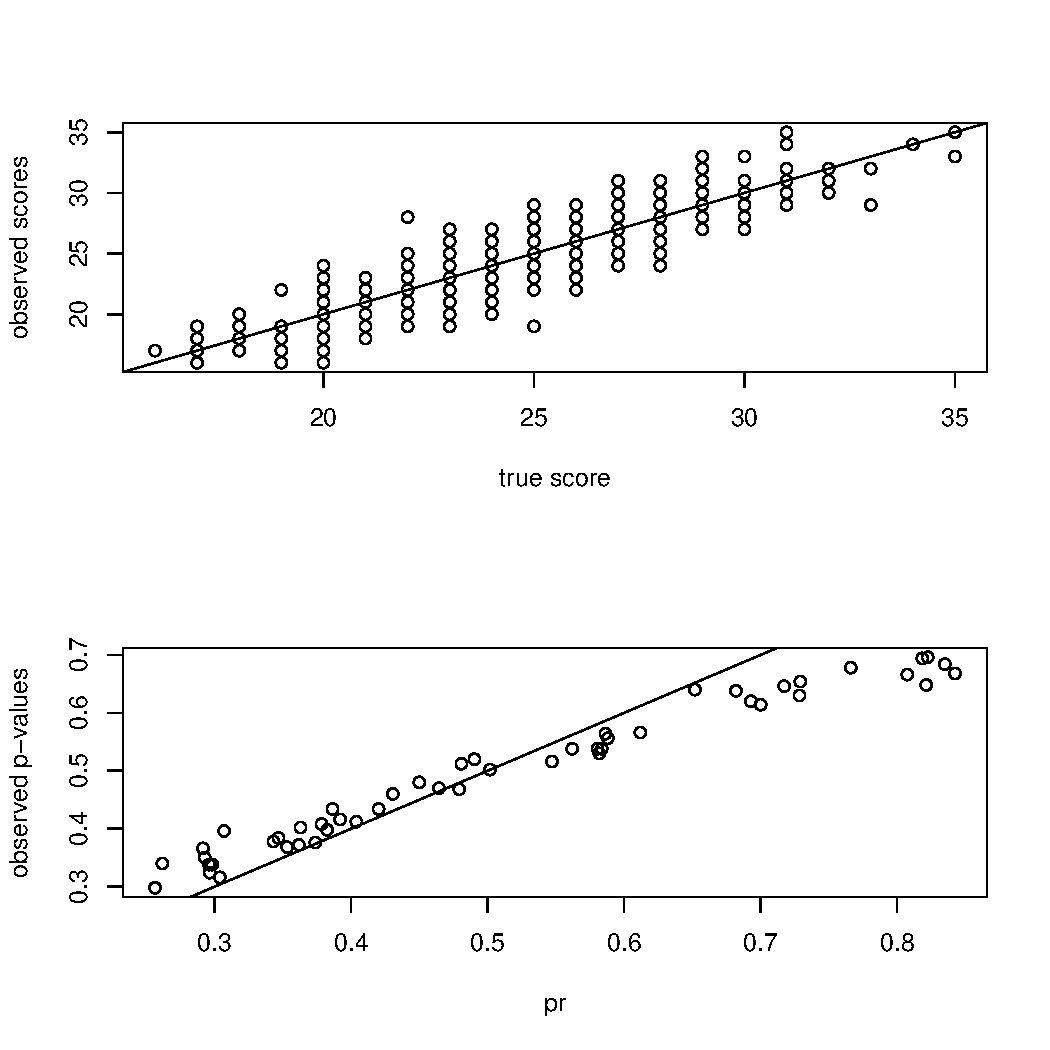
\includegraphics[width=\maxwidth]{figure/unnamed-chunk-2-8} 
\begin{kframe}\begin{verbatim}
## [1] 0.7692308 0.7870532
\end{verbatim}
\end{kframe}
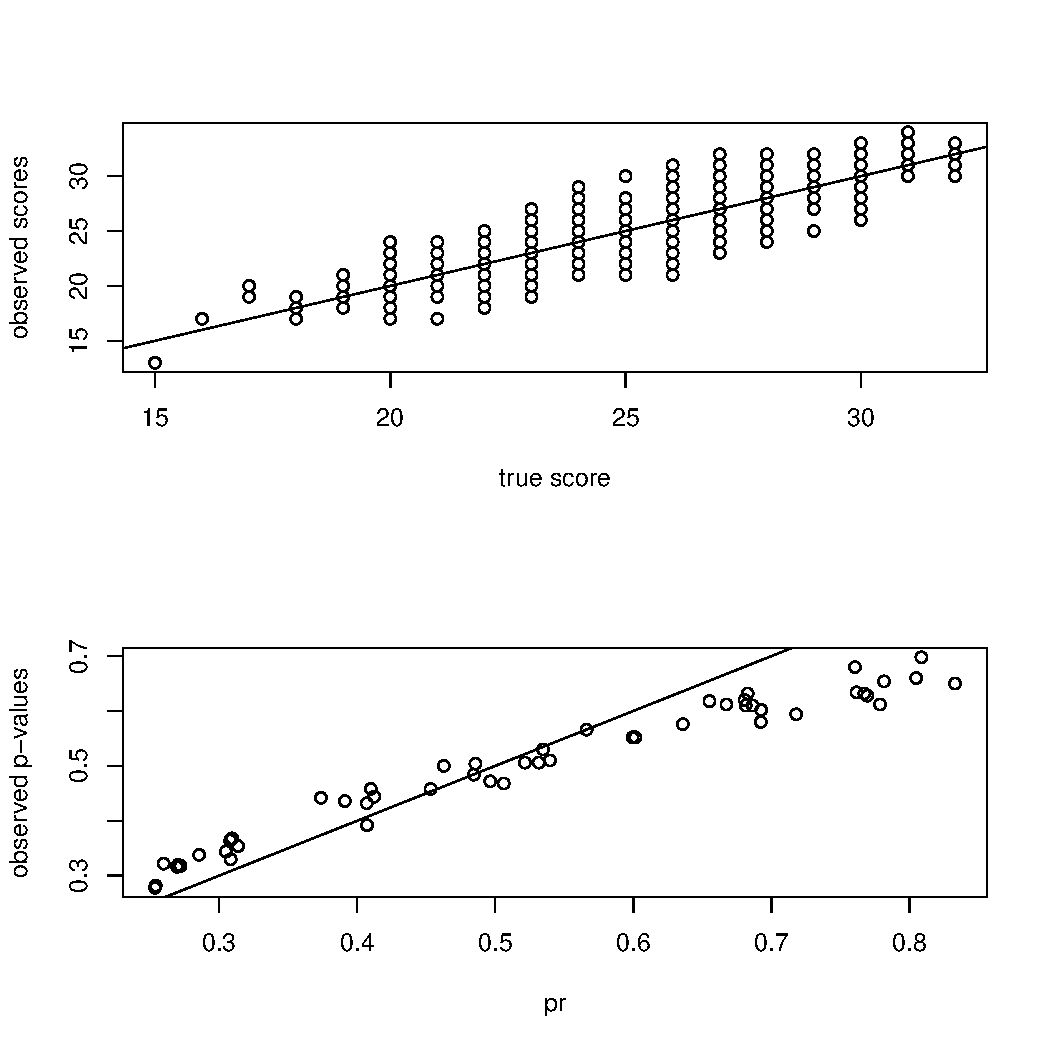
\includegraphics[width=\maxwidth]{figure/unnamed-chunk-2-9} 
\begin{kframe}\begin{verbatim}
## [1] 0.7692308 0.7521453
\end{verbatim}
\end{kframe}
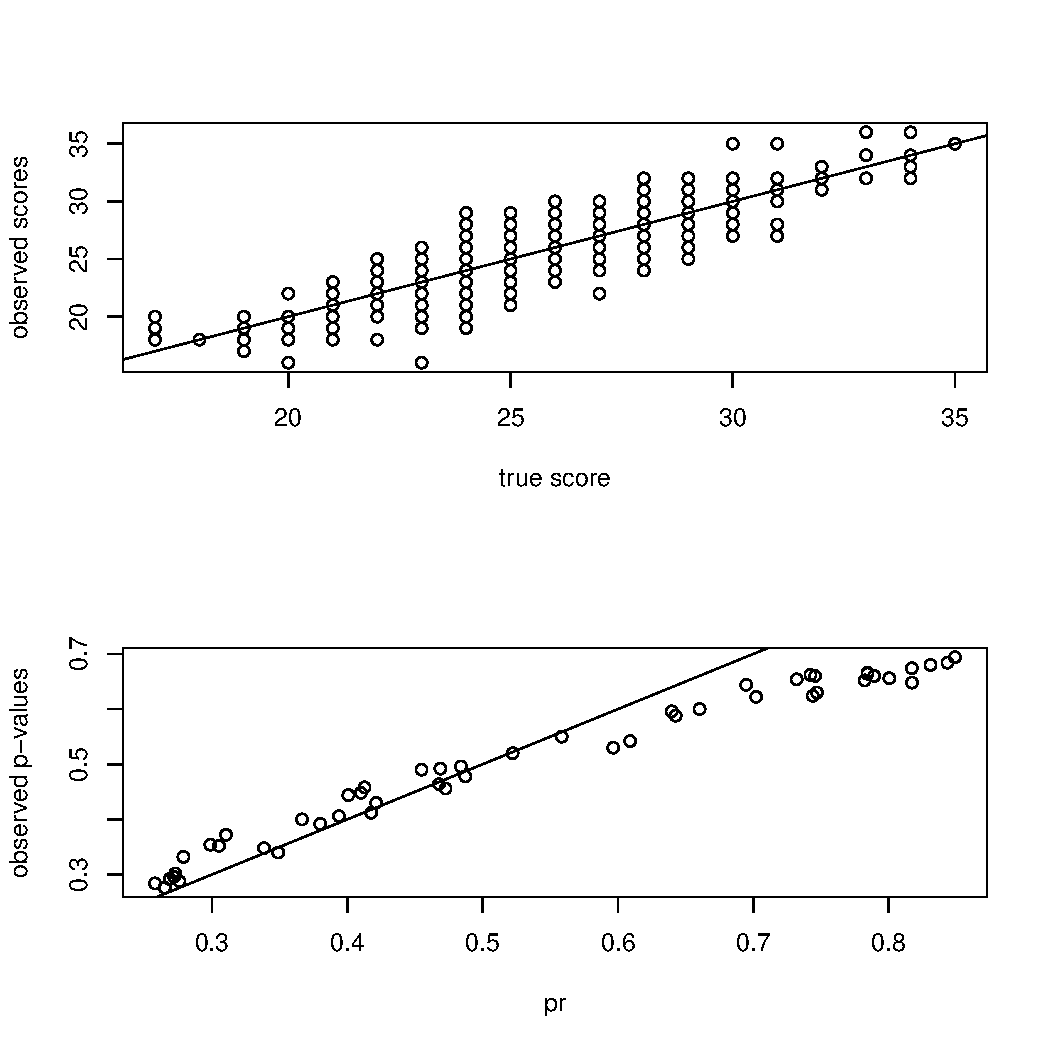
\includegraphics[width=\maxwidth]{figure/unnamed-chunk-2-10} 
\begin{kframe}\begin{verbatim}
## [1] 0.7692308 0.7601565
\end{verbatim}
\begin{alltt}
\hlkwd{do.call}\hlstd{(}\hlstr{"rbind"}\hlstd{,alph)}\hlkwb{->}\hlstd{alph}
\hlkwd{plot}\hlstd{(alph,}\hlkwc{xlim}\hlstd{=}\hlkwd{c}\hlstd{(}\hlnum{0}\hlstd{,}\hlnum{1}\hlstd{),}\hlkwc{ylim}\hlstd{=}\hlkwd{c}\hlstd{(}\hlopt{-}\hlnum{.2}\hlstd{,}\hlnum{1}\hlstd{),}\hlkwc{pch}\hlstd{=}\hlnum{19}\hlstd{,}\hlkwc{xlab}\hlstd{=}\hlstr{"true correlation"}\hlstd{,}\hlkwc{ylab}\hlstd{=}\hlstr{"kr20"}\hlstd{);} \hlkwd{abline}\hlstd{(}\hlnum{0}\hlstd{,}\hlnum{1}\hlstd{)}
\hlkwd{abline}\hlstd{(}\hlkwc{v}\hlstd{=s2.true}\hlopt{/}\hlstd{(s2.true}\hlopt{+}\hlstd{s2.error),}\hlkwc{col}\hlstd{=}\hlstr{"red"}\hlstd{)}
\hlcom{##what you can see here is that the item response datsets have the right property when it comes to the observed correlation between O and T (these correlations are the dots; the red line is the pre-specified reliability)}
\hlcom{##but, kr20 is producing reliability estimates that are *way* low}
\hlcom{##something is going disastrously awry.}
\hlcom{##q what is it? make sure you see that the true/error variances are getting handled correctly (check the print statement and related output from sim_ctt)}
\hlcom{##q: any clues as to why this is happening? what is the feature of my data generating mechanism that causes things to get all wacky?}

\hlkwd{par}\hlstd{(}\hlkwc{mfrow}\hlstd{=}\hlkwd{c}\hlstd{(}\hlnum{3}\hlstd{,}\hlnum{3}\hlstd{),}\hlkwc{mgp}\hlstd{=}\hlkwd{c}\hlstd{(}\hlnum{2}\hlstd{,}\hlnum{1}\hlstd{,}\hlnum{0}\hlstd{),}\hlkwc{mar}\hlstd{=}\hlkwd{c}\hlstd{(}\hlnum{3}\hlstd{,}\hlnum{3}\hlstd{,}\hlnum{2}\hlstd{,}\hlnum{1}\hlstd{))}
\end{alltt}
\end{kframe}
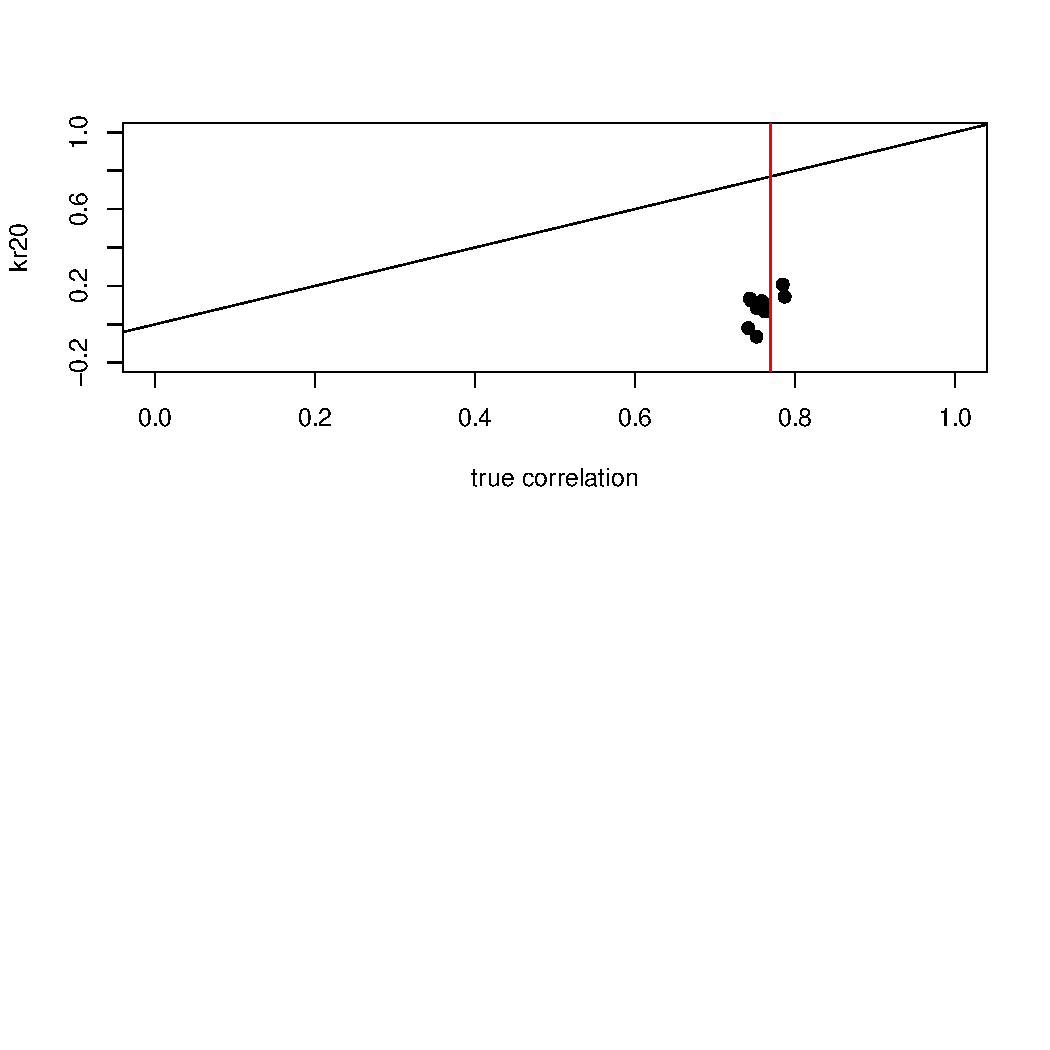
\includegraphics[width=\maxwidth]{figure/unnamed-chunk-2-11} 
\begin{kframe}\begin{alltt}
\hlcom{##now let's look at reliabilities for many different datasets generated by the above wherein we vary the true and error variances}
\hlstd{N.ppl}\hlkwb{<-}\hlnum{500}
\hlstd{N.items}\hlkwb{<-}\hlnum{50}
\hlkwa{for} \hlstd{(s2.true} \hlkwa{in} \hlstd{N.items}\hlopt{*}\hlkwd{c}\hlstd{(}\hlnum{.1}\hlstd{,}\hlnum{.5}\hlstd{,}\hlnum{.9}\hlstd{)) \{}
    \hlkwa{for} \hlstd{(s2.error} \hlkwa{in} \hlstd{N.items}\hlopt{*}\hlkwd{c}\hlstd{(}\hlnum{.1}\hlstd{,}\hlnum{.25}\hlstd{,}\hlnum{.5}\hlstd{)) \{}
        \hlstd{alph}\hlkwb{<-}\hlkwd{list}\hlstd{()}
        \hlkwa{for} \hlstd{(i} \hlkwa{in} \hlnum{1}\hlopt{:}\hlnum{10}\hlstd{) \{}
            \hlstd{alph[[i]]}\hlkwb{<-}\hlkwd{sim_ctt}\hlstd{(}\hlkwc{N.items}\hlstd{=N.items,}\hlkwc{N.ppl}\hlstd{=N.ppl,}\hlkwc{s2.true}\hlstd{=s2.true,}\hlkwc{s2.error}\hlstd{=s2.error,}\hlkwc{check}\hlstd{=}\hlnum{FALSE}\hlstd{)}
        \hlstd{\}}
        \hlkwd{plot}\hlstd{(}\hlkwd{do.call}\hlstd{(}\hlstr{"rbind"}\hlstd{,alph),}\hlkwc{xlim}\hlstd{=}\hlkwd{c}\hlstd{(}\hlopt{-}\hlnum{1}\hlstd{,}\hlnum{1}\hlstd{),}\hlkwc{ylim}\hlstd{=}\hlkwd{c}\hlstd{(}\hlopt{-}\hlnum{1}\hlstd{,}\hlnum{1}\hlstd{),}\hlkwc{pch}\hlstd{=}\hlnum{19}\hlstd{,}\hlkwc{xlab}\hlstd{=}\hlstr{"true correlation"}\hlstd{,}\hlkwc{ylab}\hlstd{=}\hlstr{"kr20"}\hlstd{)}
        \hlkwd{mtext}\hlstd{(}\hlkwc{side}\hlstd{=}\hlnum{3}\hlstd{,}\hlkwc{line}\hlstd{=}\hlnum{0}\hlstd{,}\hlkwd{paste}\hlstd{(}\hlstr{"s2.true"}\hlstd{,}\hlkwd{round}\hlstd{(s2.true,}\hlnum{2}\hlstd{),}\hlstr{"; s2.error"}\hlstd{,}\hlkwd{round}\hlstd{(s2.error,}\hlnum{2}\hlstd{)),}\hlkwc{cex}\hlstd{=}\hlnum{.7}\hlstd{)}
        \hlkwd{abline}\hlstd{(}\hlnum{0}\hlstd{,}\hlnum{1}\hlstd{)}
        \hlkwd{abline}\hlstd{(}\hlkwc{h}\hlstd{=(s2.true)}\hlopt{/}\hlstd{(s2.error}\hlopt{+}\hlstd{s2.true),}\hlkwc{col}\hlstd{=}\hlstr{"red"}\hlstd{,}\hlkwc{lty}\hlstd{=}\hlnum{2}\hlstd{)}
        \hlkwd{abline}\hlstd{(}\hlkwc{v}\hlstd{=(s2.true)}\hlopt{/}\hlstd{(s2.error}\hlopt{+}\hlstd{s2.true),}\hlkwc{col}\hlstd{=}\hlstr{"red"}\hlstd{,}\hlkwc{lty}\hlstd{=}\hlnum{2}\hlstd{)}
    \hlstd{\}}
\hlstd{\}}
\end{alltt}
\begin{verbatim}
## [1] 0.5000000 0.5128796
## [1] 0.5000000 0.5519223
## [1] 0.5000000 0.4977091
## [1] 0.5000000 0.5004587
## [1] 0.5000000 0.5330445
## [1] 0.500000 0.561126
## [1] 0.500000 0.449229
## [1] 0.5000000 0.4732625
## [1] 0.5000000 0.5281862
## [1] 0.5000000 0.5188388
## [1] 0.2857143 0.2960561
## [1] 0.2857143 0.2077476
## [1] 0.2857143 0.2754577
## [1] 0.2857143 0.3299369
## [1] 0.2857143 0.3615758
## [1] 0.2857143 0.2869029
## [1] 0.2857143 0.2856972
## [1] 0.2857143 0.3096434
## [1] 0.2857143 0.3215014
## [1] 0.2857143 0.2522629
## [1] 0.1666667 0.1409280
## [1] 0.1666667 0.1221363
## [1] 0.1666667 0.2104736
## [1] 0.1666667 0.1698770
## [1] 0.1666667 0.1679034
## [1] 0.1666667 0.1089484
## [1] 0.1666667 0.1798455
## [1] 0.1666667 0.2042687
## [1] 0.1666667 0.1583881
## [1] 0.1666667 0.1830265
## [1] 0.8333333 0.8251025
## [1] 0.8333333 0.8256566
## [1] 0.8333333 0.8443499
## [1] 0.8333333 0.8254703
## [1] 0.8333333 0.8473939
## [1] 0.8333333 0.8289805
## [1] 0.8333333 0.8364622
## [1] 0.8333333 0.8457272
## [1] 0.8333333 0.8187131
## [1] 0.8333333 0.8309489
## [1] 0.6666667 0.6557792
## [1] 0.6666667 0.6408120
## [1] 0.6666667 0.6942931
## [1] 0.6666667 0.6449742
## [1] 0.6666667 0.6748290
## [1] 0.6666667 0.6474504
## [1] 0.6666667 0.6460956
## [1] 0.6666667 0.6579885
## [1] 0.6666667 0.6462138
## [1] 0.6666667 0.6905044
## [1] 0.5000000 0.5198967
## [1] 0.5000000 0.5169372
## [1] 0.5000000 0.4533354
## [1] 0.50000 0.49399
## [1] 0.5000000 0.4506438
## [1] 0.5000000 0.5217988
## [1] 0.5000000 0.5380321
## [1] 0.5000000 0.4873121
## [1] 0.5000000 0.4506171
## [1] 0.500000 0.534523
## [1] 0.9000000 0.8853601
## [1] 0.9000000 0.9063467
## [1] 0.9000000 0.8928527
## [1] 0.9000000 0.8900774
## [1] 0.9000000 0.8951238
## [1] 0.9000000 0.8968953
## [1] 0.9000000 0.8827859
## [1] 0.9000000 0.9042878
## [1] 0.9000000 0.9132436
## [1] 0.9000000 0.9029843
## [1] 0.7826087 0.7955050
## [1] 0.7826087 0.7781482
## [1] 0.7826087 0.7762094
## [1] 0.7826087 0.8135696
## [1] 0.7826087 0.7506937
## [1] 0.7826087 0.8071848
## [1] 0.7826087 0.7963201
## [1] 0.7826087 0.7705015
## [1] 0.7826087 0.7784723
## [1] 0.7826087 0.7781468
## [1] 0.6428571 0.6429260
## [1] 0.6428571 0.6569876
## [1] 0.6428571 0.6295471
## [1] 0.6428571 0.6312202
## [1] 0.6428571 0.6329505
## [1] 0.6428571 0.6556899
## [1] 0.6428571 0.6709553
## [1] 0.6428571 0.6345450
## [1] 0.6428571 0.6440468
## [1] 0.6428571 0.6752339
\end{verbatim}
\end{kframe}
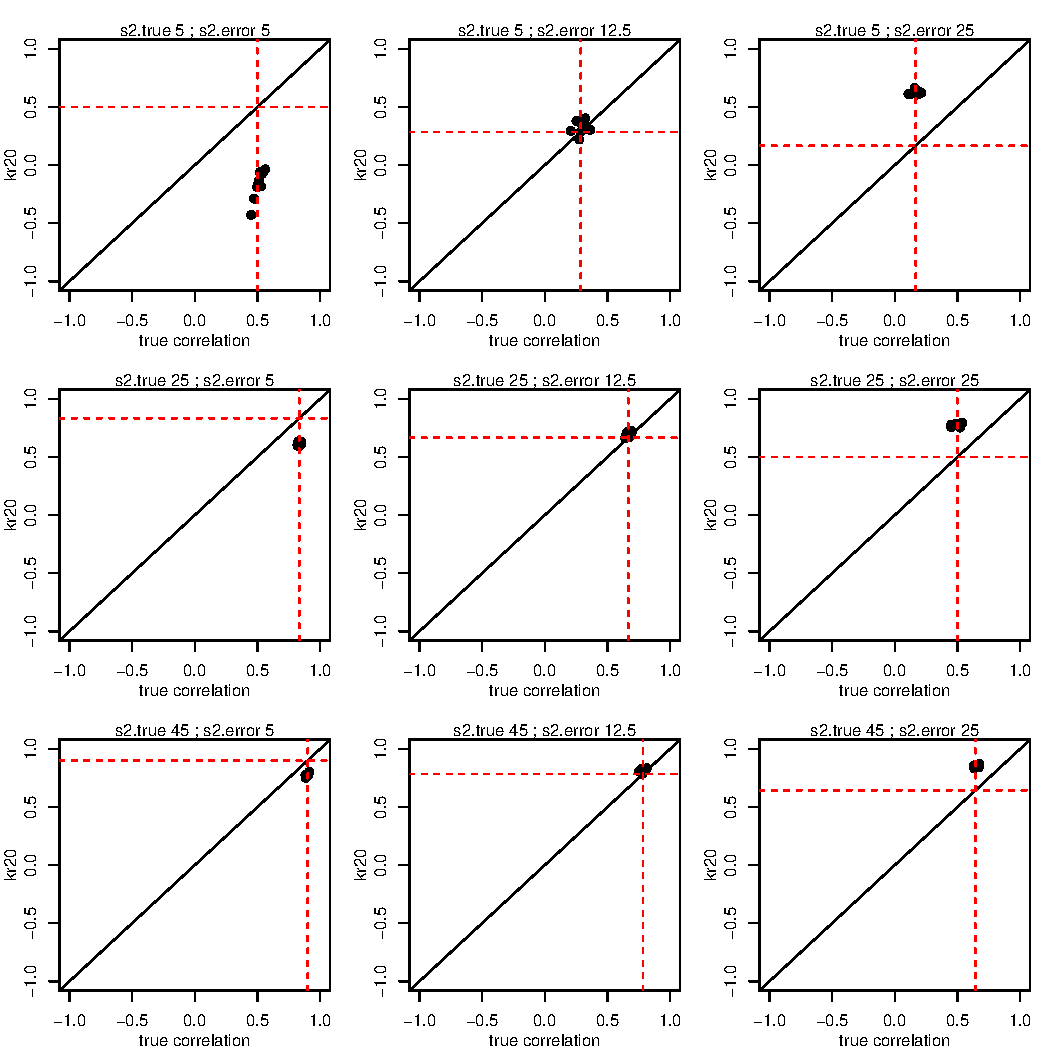
\includegraphics[width=\maxwidth]{figure/unnamed-chunk-2-12} 
\begin{kframe}\begin{alltt}
\hlcom{##q. how does the kr20 estimate of reliability behave as a function of the true and error variances?}
\hlcom{##q. what does this make you think of the CTT model? }
\end{alltt}
\end{kframe}
\end{knitrout}


\end{document}
